%%%  Bryan P Dannowitz
%%%  University of Illinois
%%%  10/19/11

\documentclass[11pt]{article}

\setlength{\topmargin}{-0.375in}
\setlength{\oddsidemargin}{-0.125in}
\setlength{\evensidemargin}{-0.125in}
\setlength{\textwidth}{6.5in}
\setlength{\textheight}{8.75in}

\usepackage{subfigure}
\usepackage{graphics}
\usepackage{wrapfig}
\usepackage{amsmath}
\usepackage{amsfonts}
\usepackage{amssymb}
\usepackage{ifpdf}

\newif\ifpdf
\ifx\pdfoutput\undefined
        \pdffalse
\else
        \pdfoutput=1
        \pdftrue
\fi

\ifpdf
        \usepackage[pdftex,
                colorlinks=true,
                urlcolor=blue,
                linkcolor=blue,
                citecolor=blue,
                ]{hyperref}
        \hypersetup{
                pdftitle={A Drell-Yan study of Short Range Correlations and the Nuclear EMC Effect at SeaQuest}
                pdfauthor={Bryan Dannowitz}
                pdfsubject={Nucleon Structure}
                pdfkeywords={EMC, Drell-Yan, Structure Functions}
                }
        \usepackage[pdftex]{graphicx}
\else
%        \usepackage[dvips]{hyperref}
\usepackage[dvips]{graphicx}

\usepackage[dvips]{graphicx,color}
\usepackage[dvipdfm]{hyperref}
\hypersetup{%
pdftitle={A Study of Transistorized Bases for the Philips XP-2008 PMT},
pdfauthor={B. Dannowitz, L. Hao},
colorlinks,linkcolor={blue},citecolor={blue},urlcolor={blue},
}%
\fi

\title{{\Large \textbf A Study of Transistorized Bases for the Philips XP-2008 PMT}}%
\author{B. Dannowitz, L. Hao\\%
  Advisor: Naomi Makins\\%
  University of Illinois At Urbana-Champaign\\%
  \href{mailto:dannowi1@illinois.edu}{\emph{dannowi1@illinois.edu}}}

\date{\normalsize{October 30th, 2012}}

\begin{document}
  \maketitle
  \begin{abstract}
In Run I of the SeaQuest experiment at Fermi National Lab, there was an indication that the photomultiplier tubes (PMT's) nearest to the target were not capable of handling periods of high-intensity, high-frequency signals from the hodoscopes. A prototype voltage divider design was chosen to improve the performance of these PMT's. These results indicate a 4x improvement in rate capability. The results also indicate a doubling of pulse amplitude, which may nullify the need for signal amplifiers for these PMT's.
  \end{abstract}

\thispagestyle{empty} 

\newpage

\tableofcontents

\newpage

\begin{figure*}
    \centerline{
    \mbox{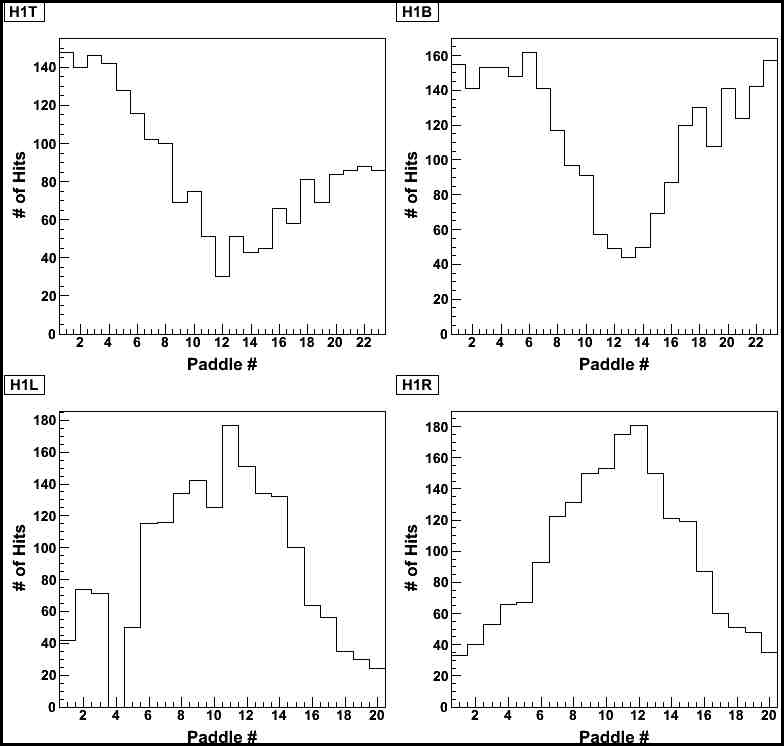
\includegraphics[width=0.5\textwidth]{nosag.jpg} 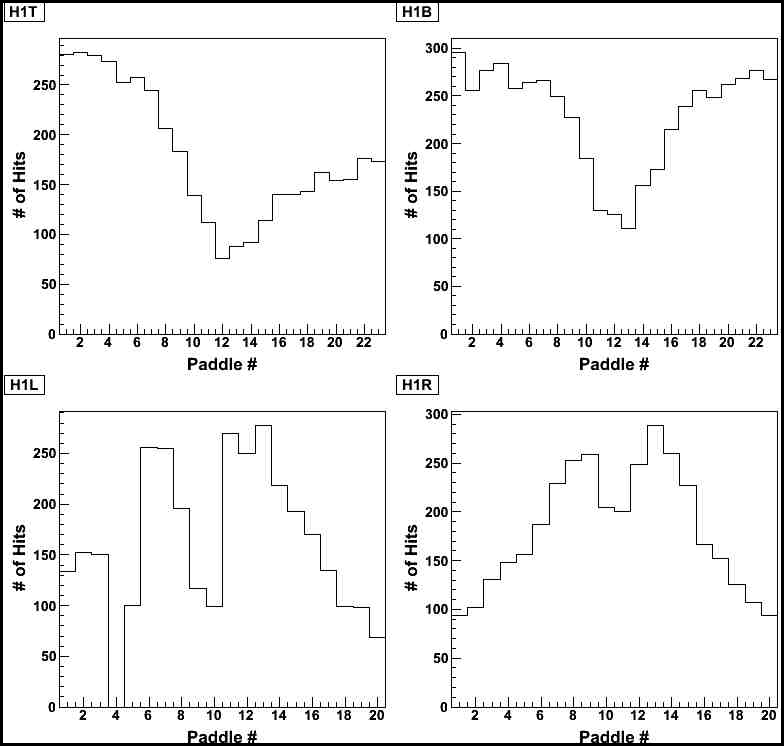
\includegraphics[width=0.5\textwidth]{sag.jpg}}
    }
    \caption{(Left) Histogram of hodoscope 'hits' in a typical event; (Right) Histogram of high-intensity event, with marked sagging in the middle of the y-measuring hodoscopes \cite{elogevidence}}
    \label{fig:sag}
\end{figure*}

\section{PMT Sagging}

During Run I of SeaQuest, it was observed on April 17th that there appeared to be a drop in expected performance in the $y-$measuring hodoscopes (Figure \ref{fig:sag}). This is assumed to be due to periods of beam reaching the NM3 enclosure being unusually intense. The result of this is pulses of light being channeled to the PMT's at an intensity and/or rate that the PMT is not capable of handling.

The understood cause of this \emph{"sag"} in performance is due to a destabilization in the voltage divider (PMT base) that holds each dynode stage at a specific voltage. When the PMT base destabilizes and is unable to maintain an appropriate voltage difference between dynode stages, this leads to inefficient performance of the PMT.

Here, we assemble a new base for our Philips XP-2008 PMT's, test several variations, and compare its performance to the original PMT base and to some Hamamatsu PMT's.

\section{PMT Bases}

\subsection{Terminology and Common Characteristics}

Each base divides -1500V over the photocathode (K), ten dynode stages (D1-D10), and the anode (A). Some common features.

There are two currents that are discussed in this document are:
\begin{itemize}
\item \textbf{Signal Current} - This is the signal that passes over the anode, which is the end-result of the cascading secondary emission electrons from each dynode stage.
\item \textbf{Bleeder Current} - This is the current through the voltage divider. It is termed the "bleeder" current since the compounding electrons in the signal current must be "bled" from the current through the voltage divider.
\end{itemize}

Throughout these voltage base designs, capacitors are commonly implemented in the latter dynode stages. These capacitors, when charged, are utilized when a large pulse of light induces a large signal current.  When this happens, the capacitors help to replenish the charge on the dynode stages without requiring the charges to be drawn from the bleeder current, thereby keeping the voltage across the dynode stages more stable.


\subsection{Original Base}

This is the PMT base that is currently used with our XP-2008 PMT's. It features capacitors of increasing capacitance along the last six stages, and steadily increases the voltage across the final four stages.

\begin{figure*}[h]
    \centerline{
    \mbox{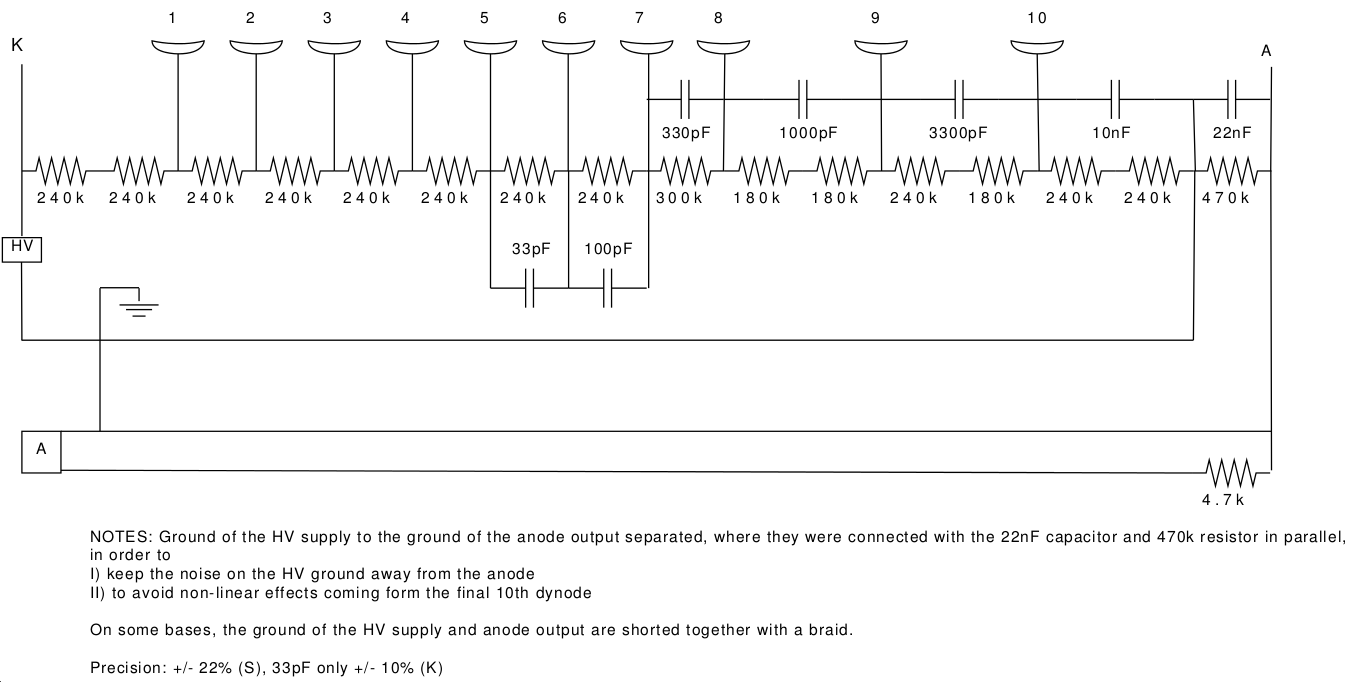
\includegraphics[width=0.75\textwidth]{pmt.png}}
    }
    \caption{The original PMT base design.}
    \label{fig:original-board}
\end{figure*}

\begin{figure*}[h]
    \centerline{
    \mbox{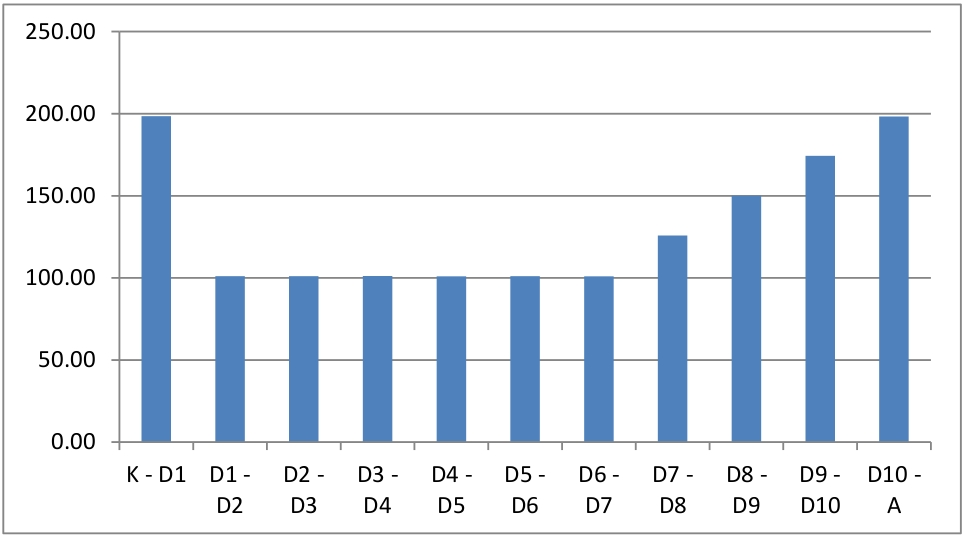
\includegraphics[width=0.75\textwidth]{original-volt.jpg}}
    }
    \caption{The (negative) voltage between subsequent stages for the original PMT base.}
    \label{fig:original-volt}
\end{figure*}

\subsection{Prototype Base v1}

This is the base design provided by Sten Hansen (Fermilab Particle Physics Division), designed in 2010 for the same model of PMT's for use at CERN. 

Three important features of this design include:

\begin{itemize}
\item
Lower resistance
\item
Parallel currents
\item
Transistors and diodes
\item
(More) Even distribution of voltage
\end{itemize}

The lower overall resistance of the voltage divider increases the bleeder current. This means that the base will be more capable of handing high-intensity/-rate events, as it will be better able to replenish the charges on each dynode stage in the case of a large signal. Typically, the larger the bleeder current, the larger the signal current can be without destabilizing the voltage divider.

At dynode six on Figure \ref{fig:v1-board}, we see that the current is split into two paths. The intent here is for the smaller current that goes through the series of $1M\Omega$ resistors maintains the voltage difference, and the larger current that freely passes through the transistors supplies the dynode stages with needed charge.

Transistors are introduced here to maintain the proper voltage division. If at any point the proper voltage drop across the gates of the transistors is not supplied (and thereby across the dynode stages), the source-to-drain current through the transistor is stopped until the proper gate voltage is restored. This helps to regulate the voltage across the dynodes, but if the charges lost to the signal current are not restored, the PMT will still eventually "sag" and fail.

The diodes are there to prevent the current from moving across the transistors improperly, and thereby preventing them from being damaged when powering the circuit on and off.

Also, the voltage across each stage, from D1 to A, are relatively flat. According to the specifications for the Philips XP-2008 photomultiplier tube, this is the recommended voltage configuration for maximum gain \cite{tubespecs}.

\begin{figure*}[h]
    \centerline{
    \mbox{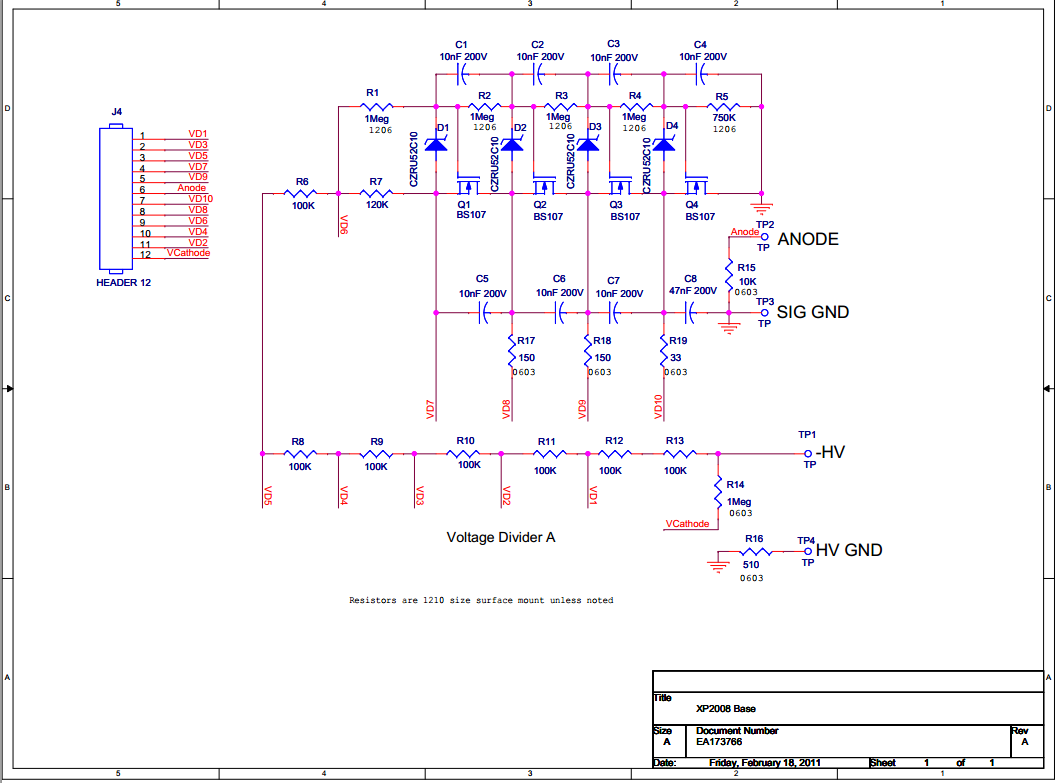
\includegraphics[width=0.7\textwidth]{newbase.png}}
    }
    \caption{The Prototype v1 board.}
    \label{fig:v1-board}
\end{figure*}

\begin{figure*}[h]
    \centerline{
    \mbox{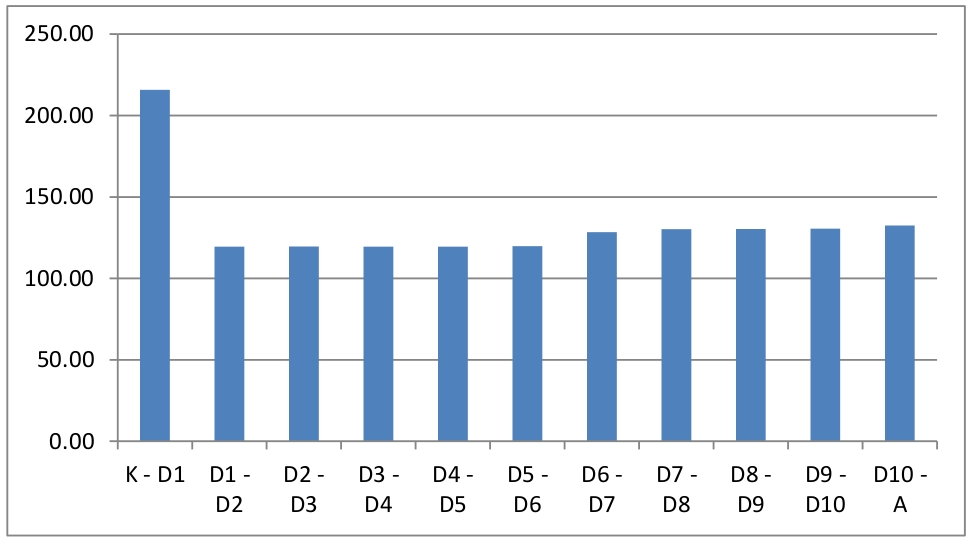
\includegraphics[width=0.75\textwidth]{v2-volt.jpg}}
    }
    \caption{The (negative) voltage between subsequent stages for the Prototype v1 PMT base.}
    \label{fig:v1-volt}
\end{figure*}
\newpage

\subsection{Prototype Base v2}

The first modification made to the prototype board was to simply halve the resistance of each of the first six stages (R6-R13 on Fig. \ref{fig:v1-board}) to increase the bleeder current.

\begin{figure*}[h]
    \centerline{
    \mbox{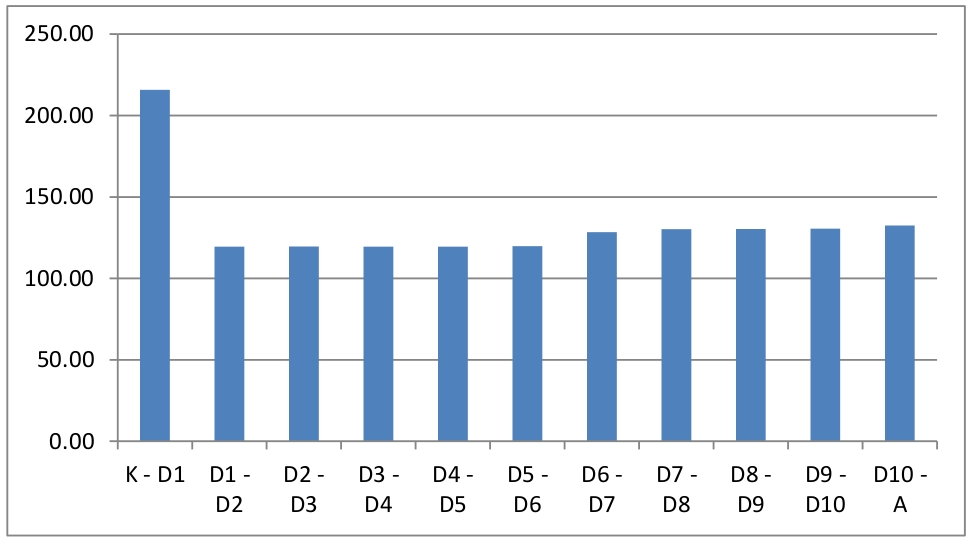
\includegraphics[width=0.75\textwidth]{v2-volt.jpg}}
    }
    \caption{The (negative) voltage between subsequent stages for the Prototype v2 PMT base.}
    \label{fig:v2-volt}
\end{figure*}
\newpage

\subsection{Prototype Base v3}

This modification "transistorized" the D5-D6 and D6-D7 stages in the case that the destabilization was ocurring even at these earlier stages (Figure \ref{fig:v3-board}).

\begin{figure*}[h]
    \centerline{
    \mbox{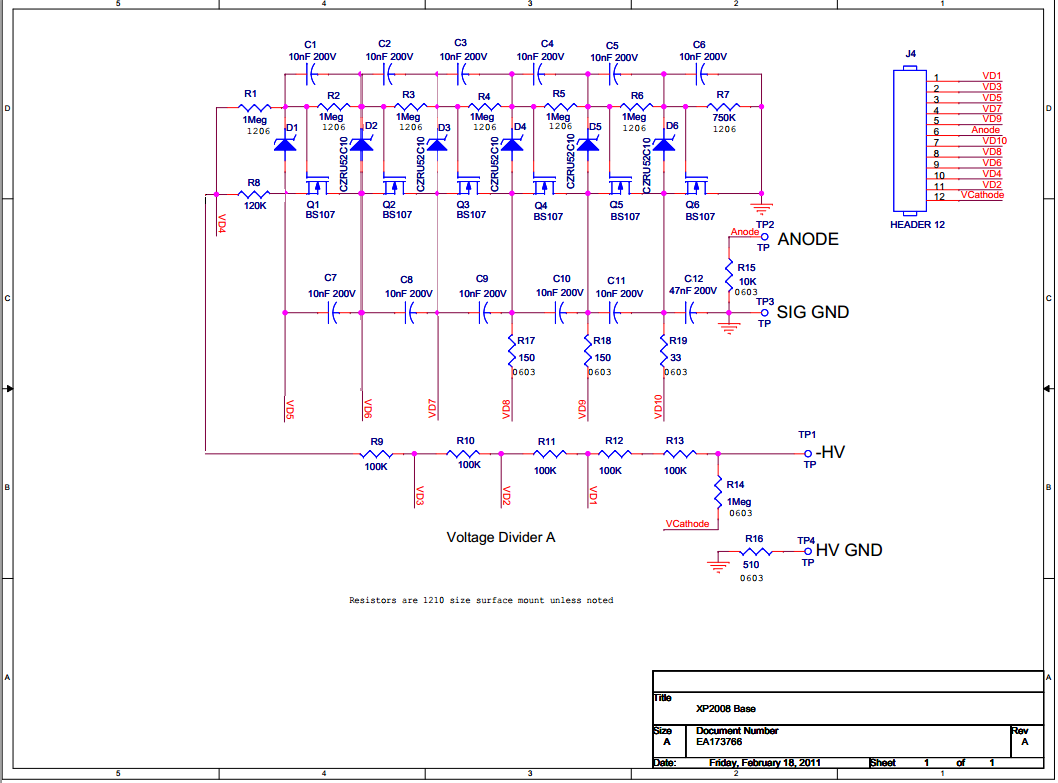
\includegraphics[width=0.75\textwidth]{newbase_6mosfet.png}}
    }
    \caption{The Prototype v3 board: 3 more transistorized stages than the Prototype v1 design.}
    \label{fig:v3-board}
\end{figure*}

\begin{figure*}[h]
    \centerline{
    \mbox{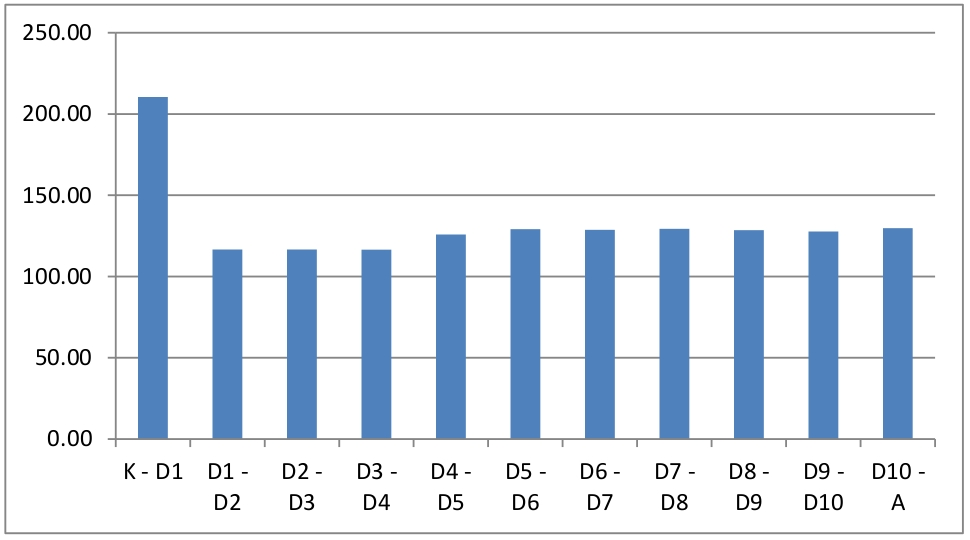
\includegraphics[width=0.75\textwidth]{v3-volt.jpg}}
    }
    \caption{The (negative) voltage between subsequent stages for the Prototype v3 PMT base.}
    \label{fig:v3-volt}
\end{figure*}
\newpage
\subsection{Prototype Base v4}

Here, the resistance over the final stage (D10-A) was increased from $1M\Omega$ to $1.5M\Omega$ (R5 in Figure \ref{fig:v1-board}). This was done in case that the final batch of electrons needed help being "swept" to the anode with a higher voltage difference.

\begin{figure*}[h]
    \centerline{
    \mbox{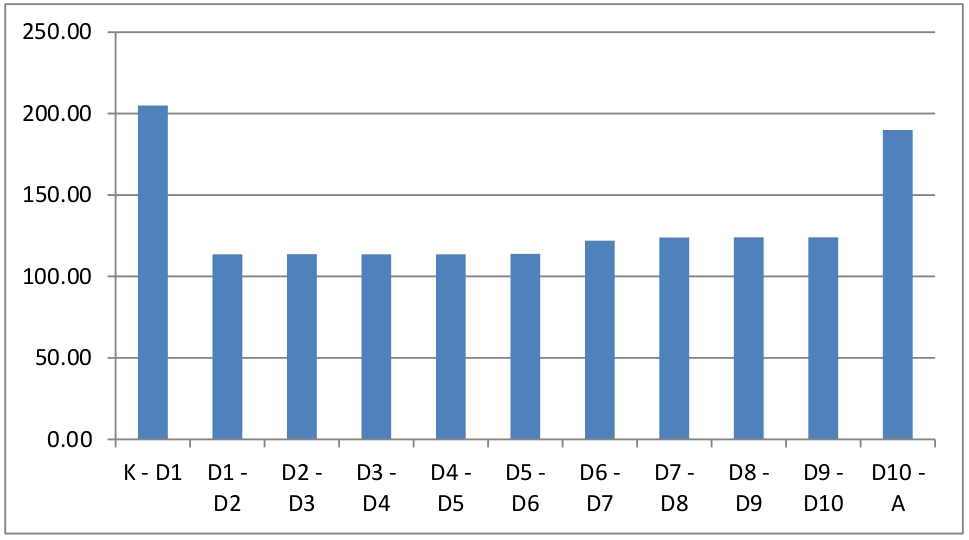
\includegraphics[width=0.75\textwidth]{v4-volt.jpg}}
    }
    \caption{The (negative) voltage between subsequent stages for the Prototype v4 PMT base.}
    \label{fig:v4-volt}
\end{figure*}
\newpage

\section{PMT Base Comparisons}

There is a specific difficulty with the objective to increase the rate capability of our PMT's. This difficulty is that we do not have a target rate to attain. The rate and intensity that caused the original PMT+base to sag is unknown, and if it was known, it would be difficult to match the intensity with an experimental setup.

As a result, the objective in these tests is to \emph{compare} the performance of the same PMT using different bases.

\subsection{Testing Apparatus and Measurments}

In this experiment, a PMT attached to a PMT base is placed into a light-tight box along with an fast-pulsing LED. 

The LED is driven by an Agilent function generator capable of generating signals up to 30MHz. The LED's intensity is attenuated by a neutral density filter (NDF), with a rating D=3.0, where the NDF allows 1 in $10^D$ photons through (1 in 1000 for D=3.0).

The PMT base is powered by a high voltage supply with an ammeter between the two in order to measure the bleeder current. The PMT signal is processed 

\begin{figure*}[h]
    \centerline{
    \mbox{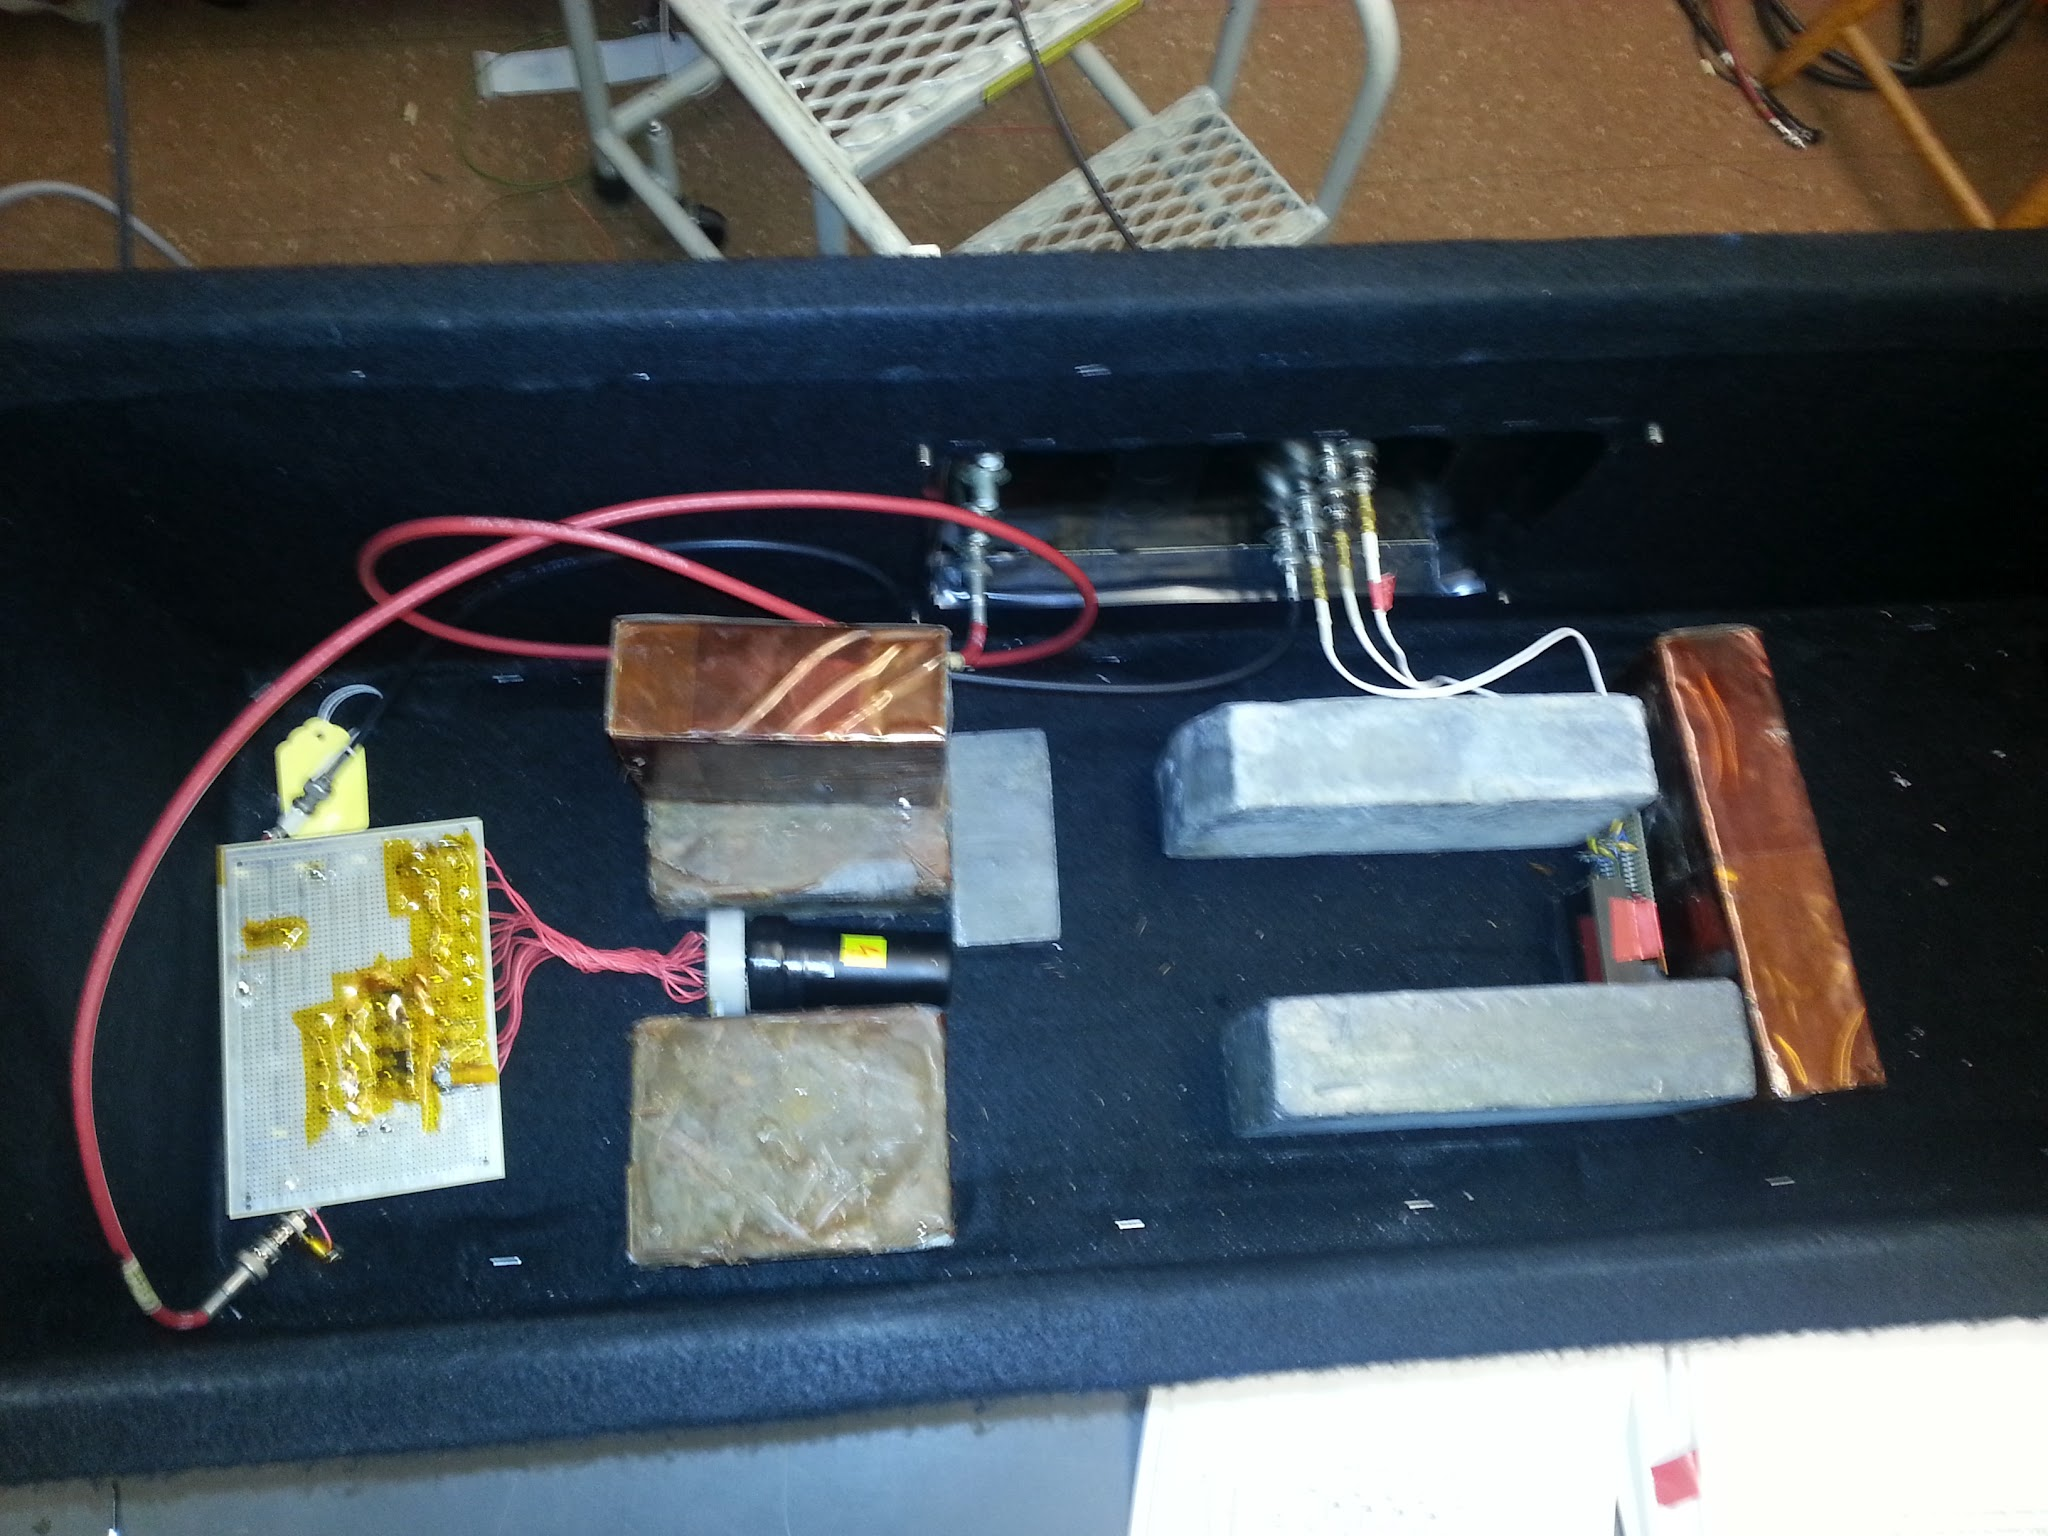
\includegraphics[width=0.75\textwidth]{setup.jpg}}
    }
    \caption{Inside of a lightbox, we have our prototype board (left) wired up to a Philips XP-2008 PMT (middle), facing a fast-led source (right) }
    \label{fig:setup}
\end{figure*}

\subsection{Test 1: Original Base vs. Prototype Board v1}


\subsection{Test 2: Original Base vs. Prototype Board v1 (With Bleeder Current)}


\subsection{Test 3: Original Base vs. Prototype v1 vs. Prototype v2}


\subsection{Test 4: Prototype v1 vs. Prototype v3}


\subsection{Test 5: Prototype v1 vs. Prototype v4}


\subsection{Test 6: Hamamatsue Bases}

\subsection{Test 7: NDF D=3.0 vs NDF D=4.0}


\section{Conclusions}


\bigskip
\bibliography{Dannowitz_PMT_Study}
\bibliographystyle{plain}

\end{document}